\clearpage
\begingroup
\setlength{\intextsep}{6pt}
\captionsetup{skip=3pt,font=small}
\section{Additional model error evidence}
Seed 42 F1-selected checkpoints complement the CNN analysis on the same 6,000 validation images. Examples show the first three correct IDs and three largest true-label NLL errors; they illustrate behavior rather than estimate its frequency.
\subsection{Linear: validation errors and examples}
Recipe C1, seed 42, selected epoch 40: accuracy 86.850\%, macro-F1 86.876\%. Each true class contributes 600 images. The largest off-diagonal counts are 
Shirt $\rightarrow$ T-shirt: 78/600 (13.00\%); Pullover $\rightarrow$ Coat: 70/600 (11.67\%); Coat $\rightarrow$ Shirt: 62/600 (10.33\%).
\begin{figure}[H]\centering
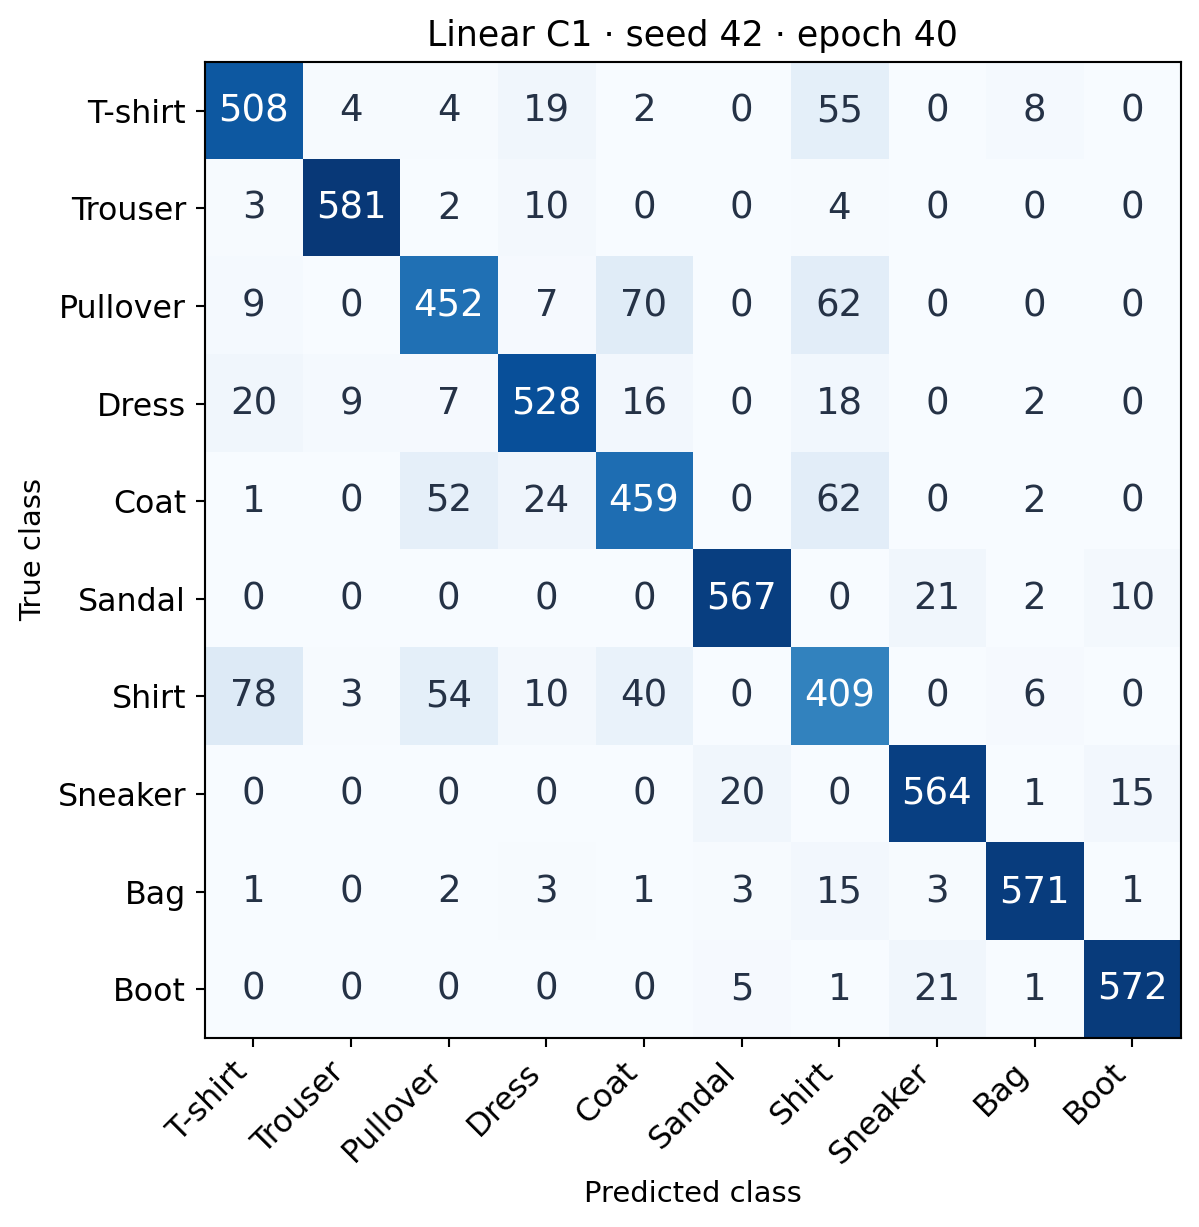
\includegraphics[width=0.60\linewidth]{appendix_figures/linear_seed42_confusion.png}
\caption{Linear integer confusion counts on old validation.}
\end{figure}
\begin{figure}[H]\centering
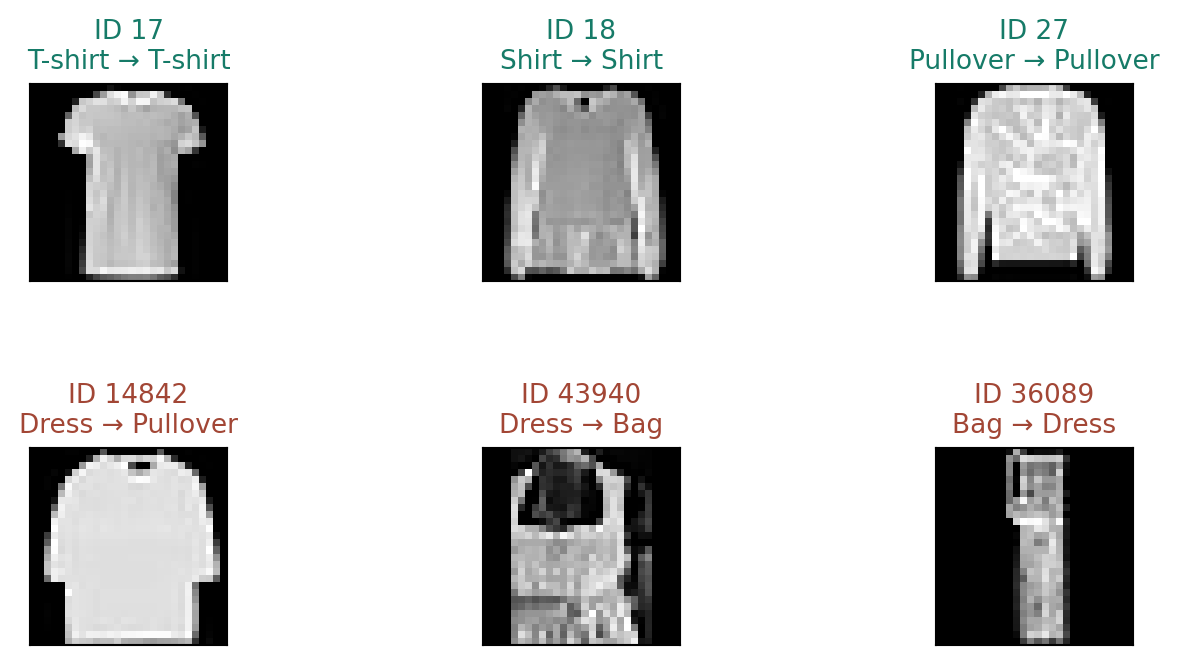
\includegraphics[width=0.68\linewidth]{appendix_figures/linear_seed42_examples.png}
\caption{Linear examples: first three correct IDs (top), three highest-NLL errors (bottom). Titles give true and predicted labels.}
\end{figure}
\clearpage
\subsection{MLP: validation errors and examples}
Recipe C7, seed 42, selected epoch 56: accuracy 91.500\%, macro-F1 91.501\%. Each true class contributes 600 images. The largest off-diagonal counts are 
Shirt $\rightarrow$ T-shirt: 56/600 (9.33\%); T-shirt $\rightarrow$ Shirt: 48/600 (8.00\%); Pullover $\rightarrow$ Coat: 45/600 (7.50\%).
\begin{figure}[H]\centering
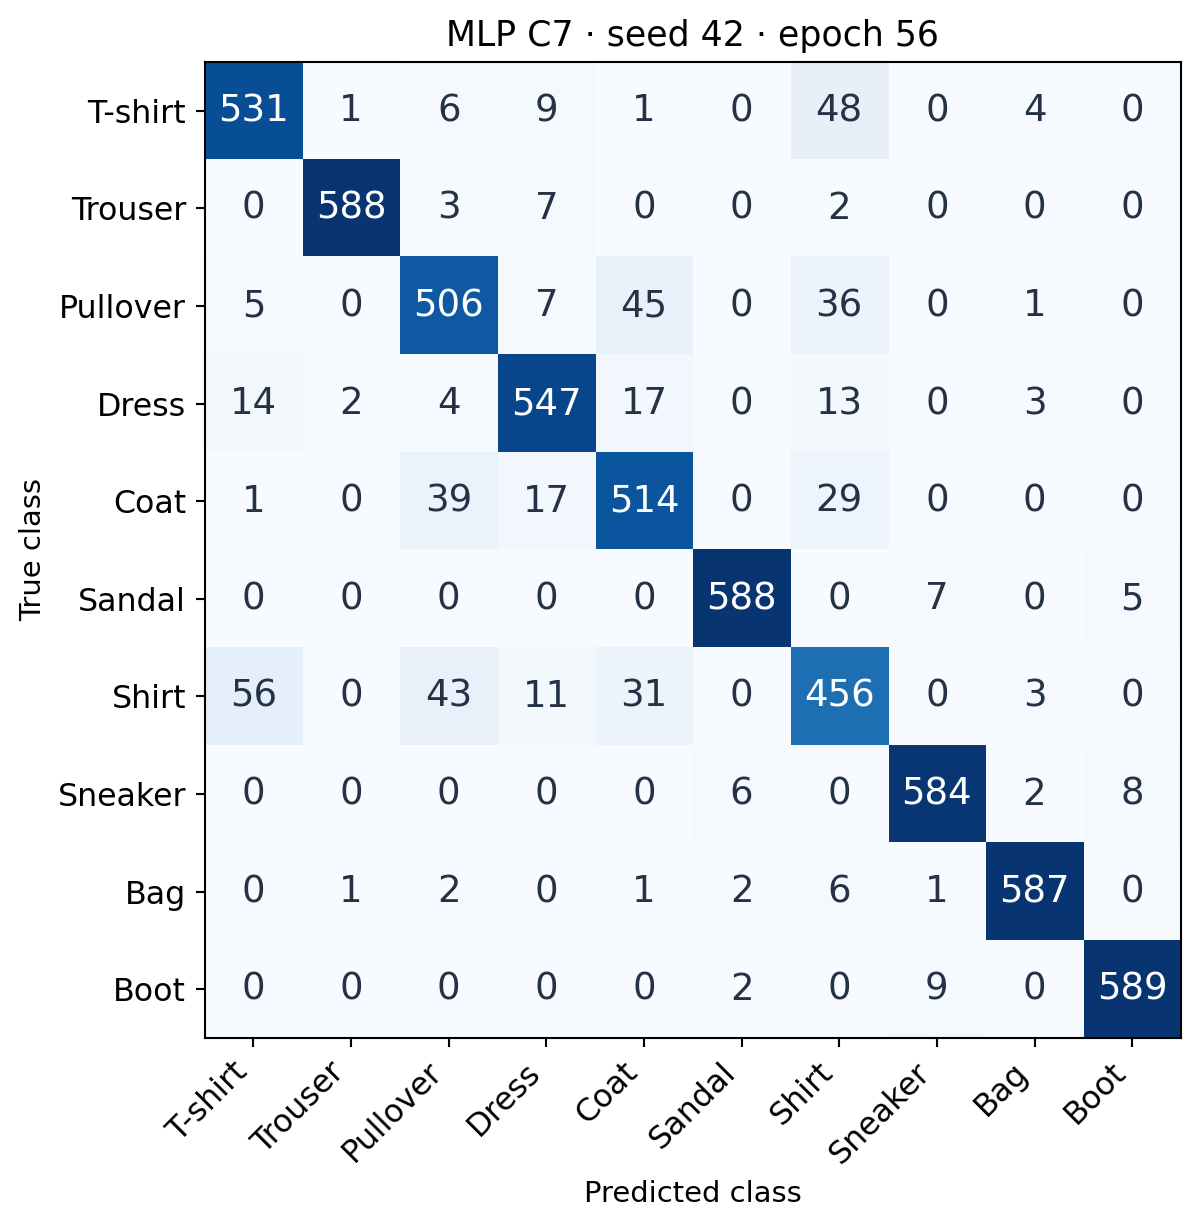
\includegraphics[width=0.60\linewidth]{appendix_figures/mlp_seed42_confusion.png}
\caption{MLP integer confusion counts on old validation.}
\end{figure}
\begin{figure}[H]\centering
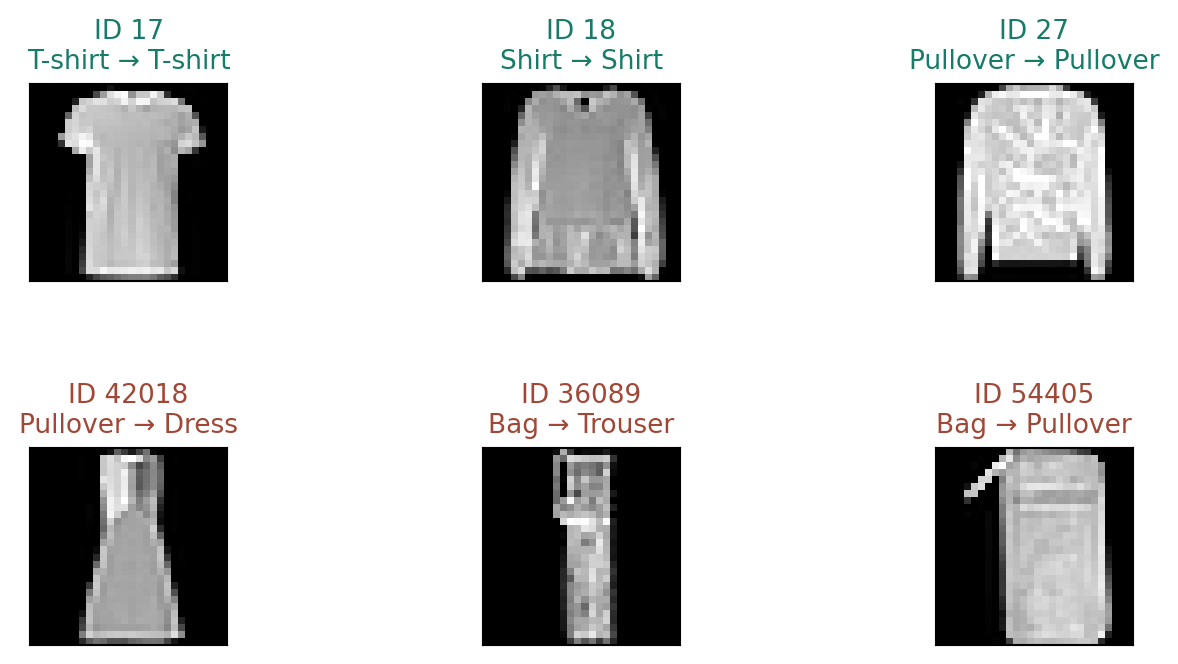
\includegraphics[width=0.68\linewidth]{appendix_figures/mlp_seed42_examples.png}
\caption{MLP examples: first three correct IDs (top), three highest-NLL errors (bottom). Titles give true and predicted labels.}
\end{figure}
\clearpage
\subsection{GRU: validation errors and examples}
Recipe C1, seed 42, selected epoch 37: accuracy 91.350\%, macro-F1 91.324\%. Each true class contributes 600 images. The largest off-diagonal counts are 
Shirt $\rightarrow$ T-shirt: 59/600 (9.83\%); T-shirt $\rightarrow$ Shirt: 52/600 (8.67\%); Pullover $\rightarrow$ Coat: 46/600 (7.67\%).
\begin{figure}[H]\centering
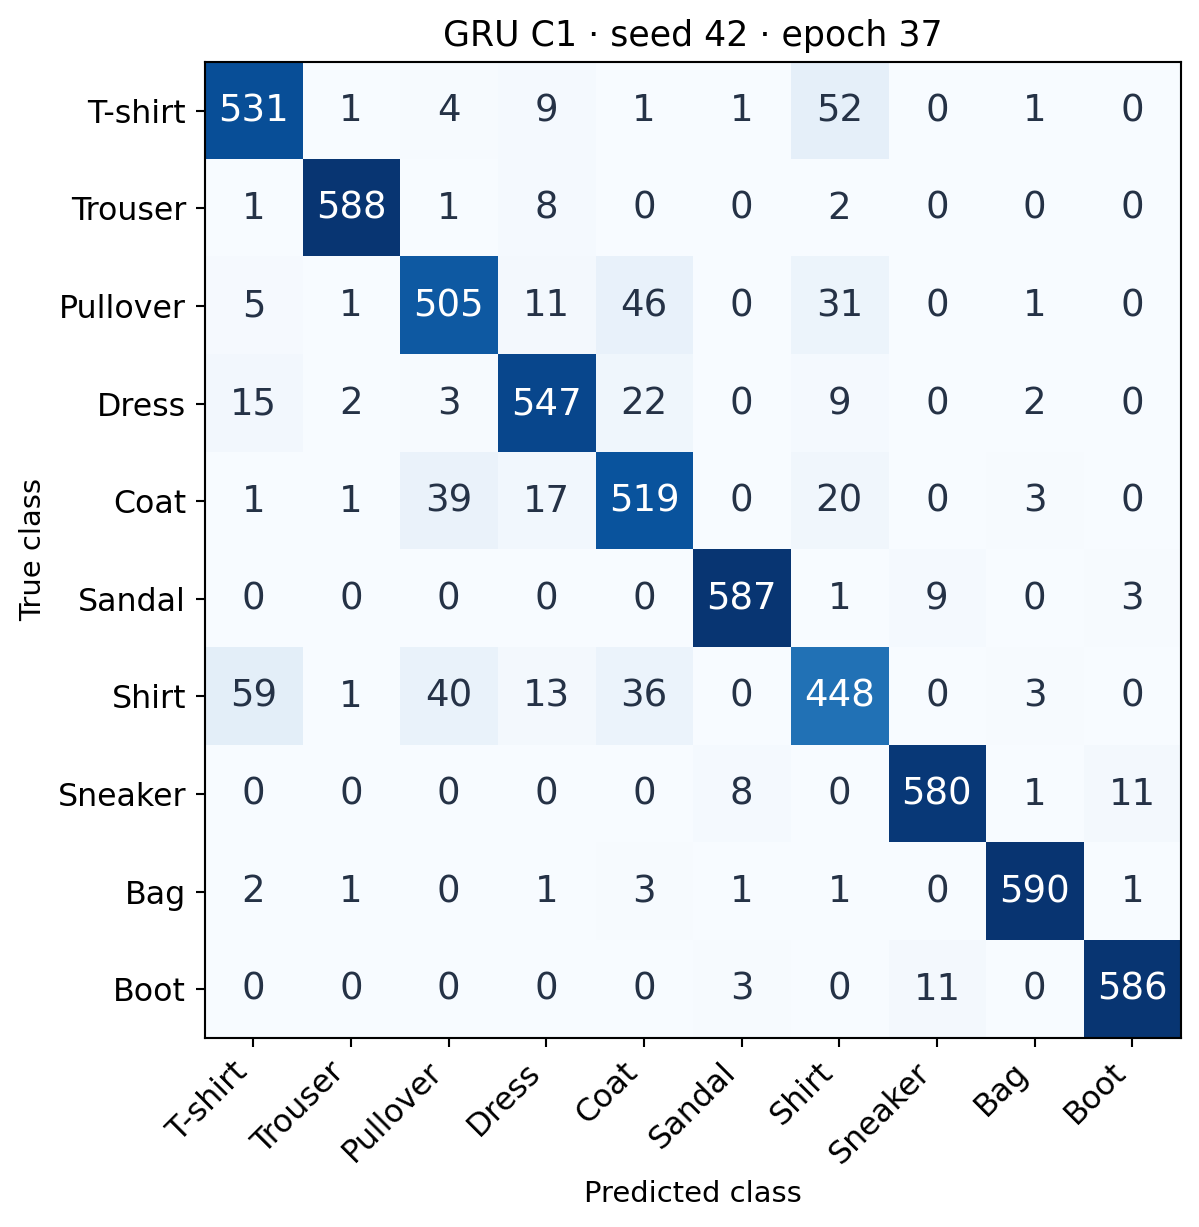
\includegraphics[width=0.60\linewidth]{appendix_figures/gru_seed42_confusion.png}
\caption{GRU integer confusion counts on old validation.}
\end{figure}
\begin{figure}[H]\centering
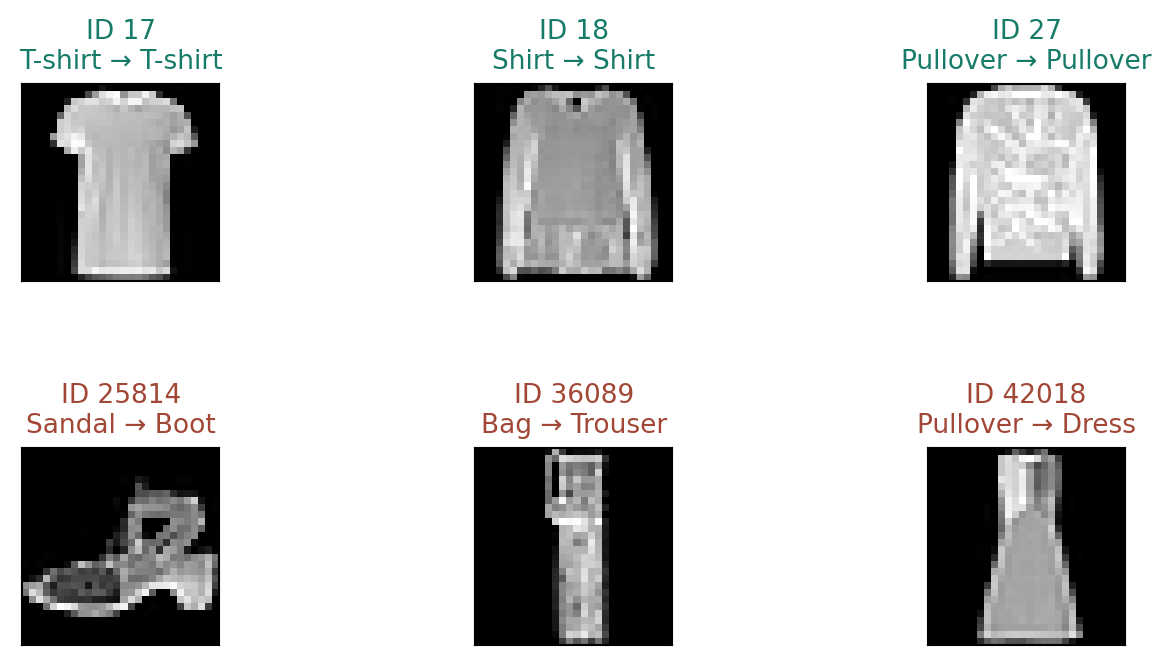
\includegraphics[width=0.68\linewidth]{appendix_figures/gru_seed42_examples.png}
\caption{GRU examples: first three correct IDs (top), three highest-NLL errors (bottom). Titles give true and predicted labels.}
\end{figure}
\clearpage
\subsection{Transformer: validation errors and examples}
Recipe C1, seed 42, selected epoch 58: accuracy 91.567\%, macro-F1 91.541\%. Each true class contributes 600 images. The largest off-diagonal counts are 
Shirt $\rightarrow$ T-shirt: 54/600 (9.00\%); T-shirt $\rightarrow$ Shirt: 41/600 (6.83\%); Coat $\rightarrow$ Pullover: 39/600 (6.50\%).
\begin{figure}[H]\centering
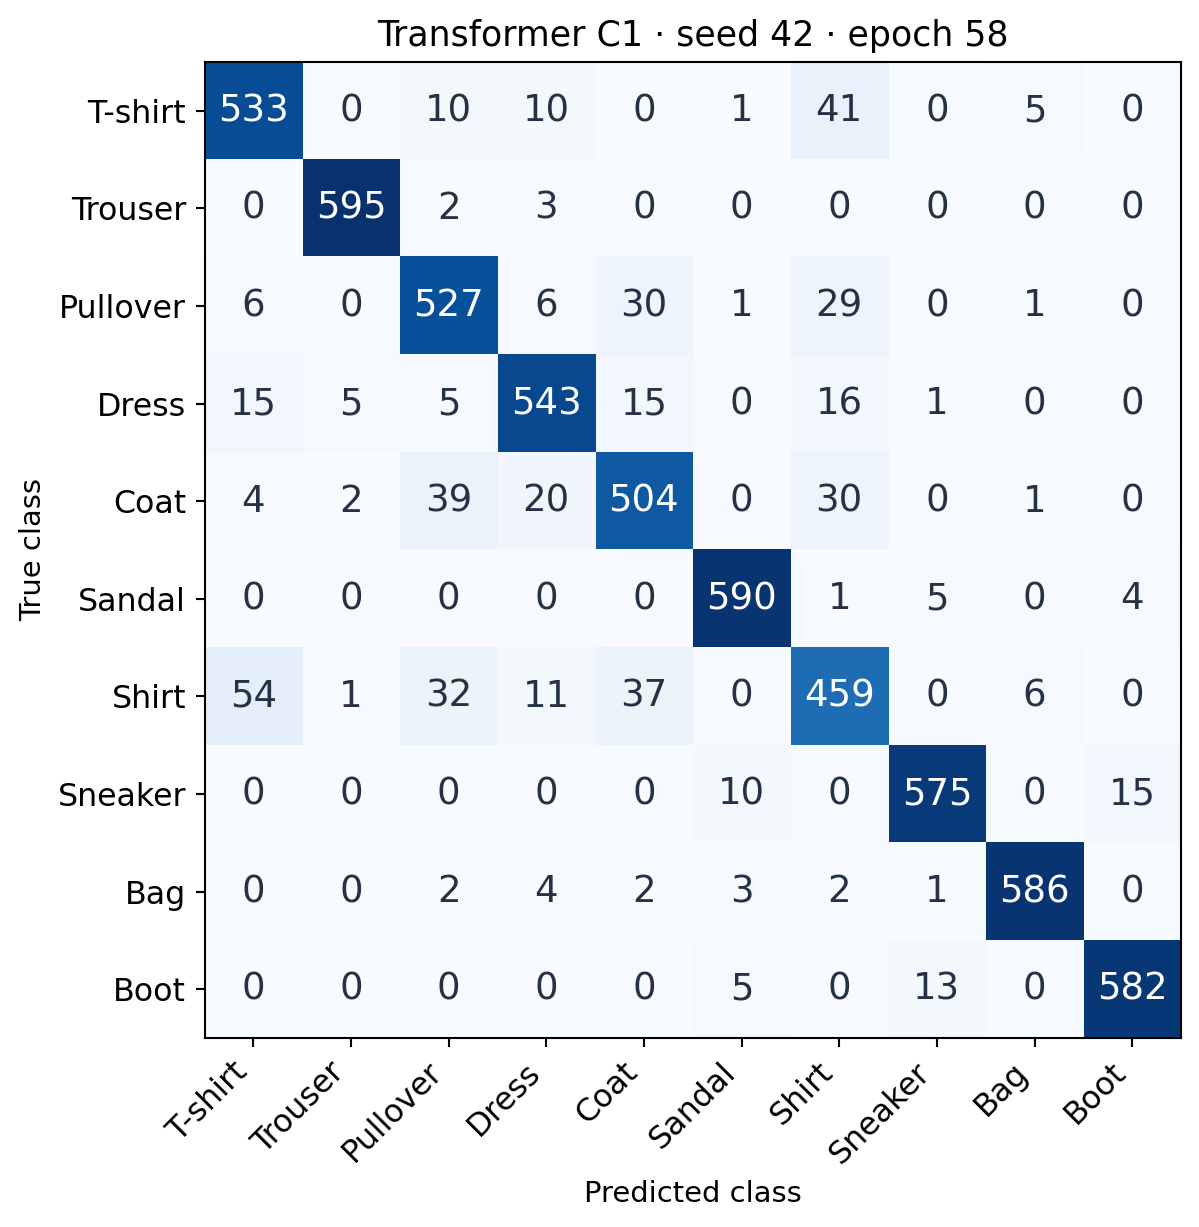
\includegraphics[width=0.60\linewidth]{appendix_figures/transformer_seed42_confusion.png}
\caption{Transformer integer confusion counts on old validation.}
\end{figure}
\begin{figure}[H]\centering
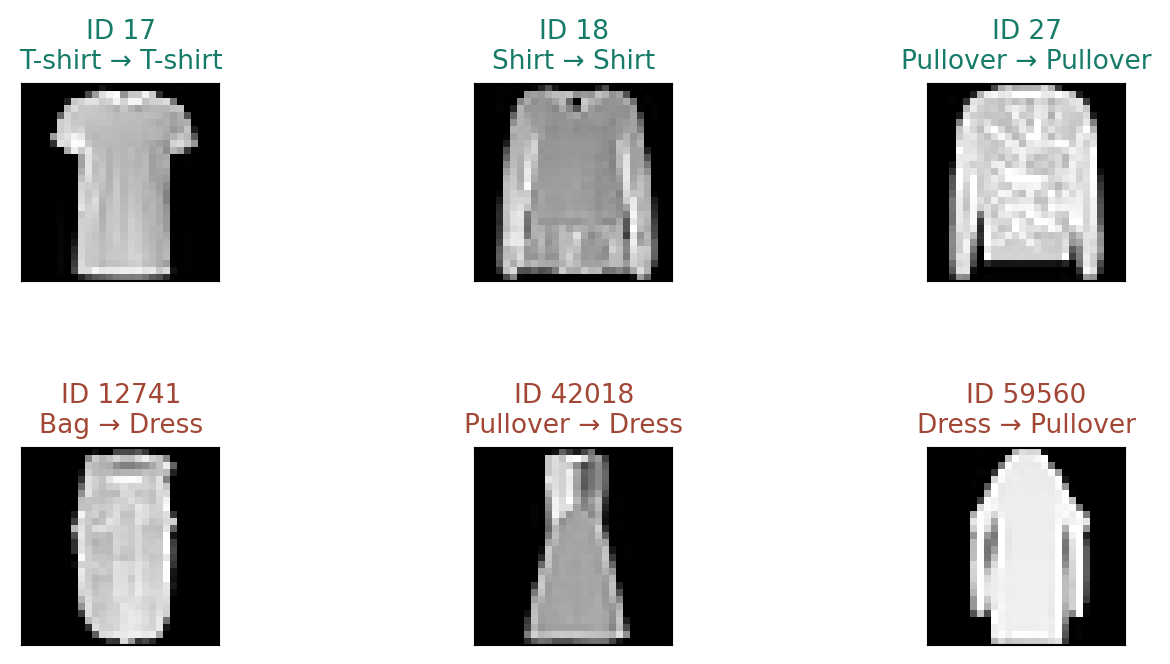
\includegraphics[width=0.68\linewidth]{appendix_figures/transformer_seed42_examples.png}
\caption{Transformer examples: first three correct IDs (top), three highest-NLL errors (bottom). Titles give true and predicted labels.}
\end{figure}
\endgroup
